\documentclass{article}
\usepackage{graphicx}
\usepackage{cite}
\usepackage{amsmath}

\title{Assignment 4}
\author{Jahaan Shah}
\date{June 2023}

\begin{document}

\section{AE22B105}

\textbf{Name:} Jahaan Shah \\
\textbf{GitHub User ID:} jahaanshahae22b105

\subsection{Equation and Description}

The equation I've chosen is the Schrödinger-Poisson Equation, which combines the Schrödinger equation from quantum mechanics with the Poisson equation from electrostatics. The Schrödinger-Poisson Equation is given by:

\begin{equation}
-\frac{{\hbar^2}}{{2m}} \nabla^2 \Psi + V(\mathbf{r})\Psi = E\Psi
\end{equation}

\begin{equation}
\nabla^2 V = \frac{{-e}}{{\varepsilon_0}}(N_D - N_A + p - n)
\end{equation}


\begin{quote}
    
In this equation:

\begin{itemize}
\item
  \begin{quote}
  $\psi$ represents the wave function of a quantum system.
  \end{quote}
\item
  \begin{quote}
  $\nabla^2$ is the Laplacian operator, representing the spatial variation of
  the wave function.
  \end{quote}
\item
  \begin{quote}
  V is the potential energy function.
  \end{quote}
\item
  \begin{quote}
  q represents the elementary charge.
  \end{quote}
\item
  \begin{quote}
  n represents the electron density.
  \end{quote}
\item
  \begin{quote}
  $N_\text{a}^+$ represents the density of positively charged ions.
  \end{quote}
\item
  \begin{quote}
  $N_\text{a}^-$ represents the density of negatively charged ions.
  \end{quote}
\item
  \begin{quote}
  $\varepsilon_0$ is the permittivity of free space.
  \end{quote}
\end{itemize}

\end{quote}
The Schrödinger-Poisson Equation\cite{lange1995overview} describes the behavior of charged particles in a semiconductor device under the influence of both quantum mechanical effects (represented by the Schrödinger equation) and electrostatic interactions (represented by the Poisson equation). It provides a framework for analyzing the electronic properties and carrier transport in semiconductor devices such as transistors and diodes.

This equation is of significant importance in the field of semiconductor physics\cite{pierret1996semiconductor} and device engineering. It is commonly used to design and optimize electronic devices, understand quantum transport phenomena, and develop computational models for semiconductor simulations.

I looked up this equation and its description from various sources, including textbooks on solid-state physics and semiconductor device physics.

\subsection{Images}

\begin{figure}
    \centering
    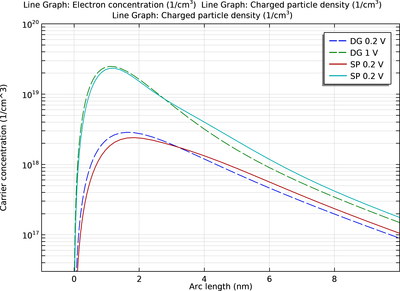
\includegraphics[width=0.5\textwidth]{image.png}
    \caption{Electron density distribution in a semiconductor device}
    \label{fig:image9}
\end{figure}

Figure \ref{fig:image9} shows a visualization of the electron density distribution in a semiconductor device, illustrating the concept described by the Schrödinger-Poisson Equation.




\bibliography{bibliography}
\bibliographystyle{plain}

\end{document}
